\chapter{Design and Analysis of the Dental Surgical Robot -- DentiBot}
\label{chapter3}
\hspace*{6mm}To design a autonomous endodontic robot, its workspace and dimension are discussed in Section \ref{sec:requirement} followed by detail description of hardware of DentiBot in Section \ref{sec: design of dentibot}. Technical solutions to system integration with a robot arm are clarified in this chapter. Section \ref{sec:kinematics} and Section \ref{sec:ref_robot} serve as a robot arm tutorial and provide some imperative approaches when combining a robot arm and an end effector.
\section{Requirement and Specification}
\label{sec:requirement}
\hspace*{6mm}The dental surgical robot should perform delicate and complicated surgery operations because the average diameter of a root canal is $0.28\ (\pm 0.08)$ mm \cite{wu2002does}. Therefore, our system should have a high resolution of movement. Next, an appropriate workspace is required. In dental anatomy, teeth are located on the maxillary (lower jaw) and the mandibular (upper jaw). To perform surgery with both sides, the end effector should rotate at least $180$ degrees. Furthermore, a research indicated that the average range of maximum mouth opening is 50.3 (±6.26) mm \cite{agrawal2015evaluation}. Hence, the end effector should be less than this range.
\section{Design of DentiBot}
\label{sec: design of dentibot}
\vspace{-5mm}
\hspace*{6mm}As discussed in the previous section, we decide to build a system composed of a robot arm, an F/T sensor, and a modified handpiece. Why choosing a robot arm and an F/T sensor is because we want to mimic the dentist's clinical behaviour. Due to the 6-DOF robot arm, DentiBot can achieve the action with less hardware restriction. DentiBot can easily move to almost desired positions and rotate more than $180$ degrees to drill tooth in both sides of mouth. Also, with the 6-DoF F/T sensor, the real-time force and torque feedbacks are obtained and serve as a haptic feedback. DentiBot can take reaction with the F/T sensor such as a dentist touch and sense something in the surgery and do the corresponding reaction. Besides, by modifying the existing handpiece, which is a handheld dental electric device, there is no doubt that the workspace and dimension in the mouth are satisfied. Also, there are two adapters designed to assemble these devices.
\par
\begin{figure}[htbp]
\begin{center}
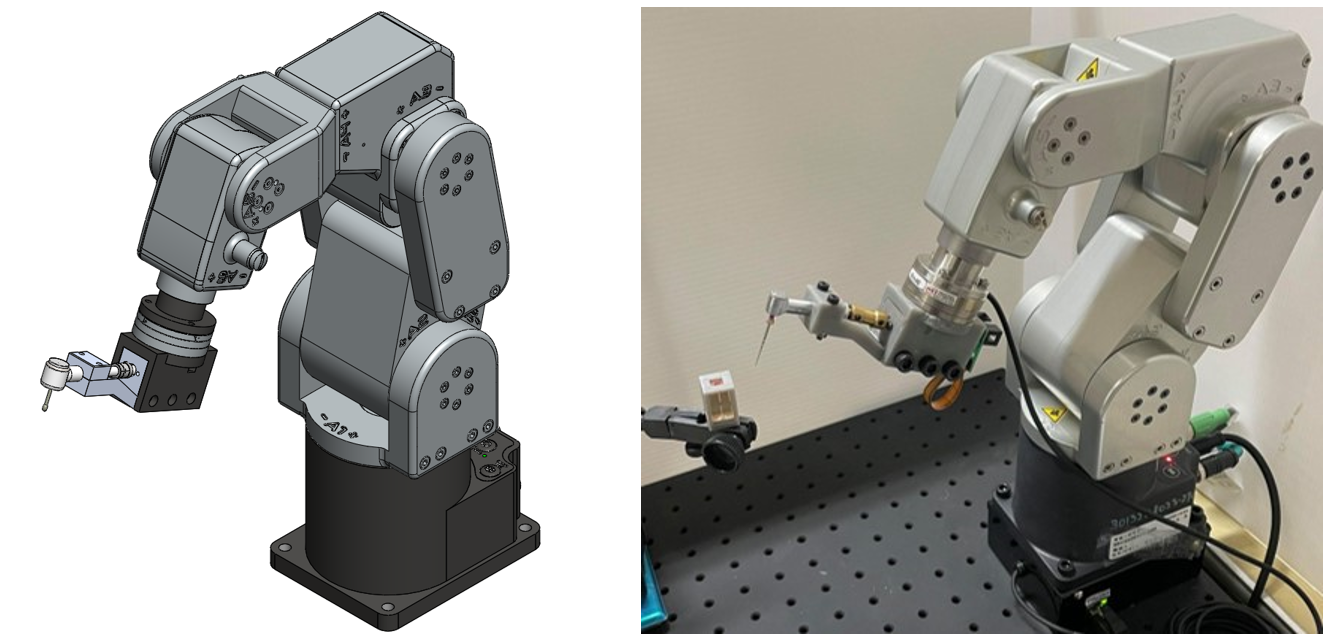
\includegraphics[width=1\linewidth]{Images/DentiBot.png}
\caption{
DentiBot formed by a 6 DoF robotic manipulator
}\label{fig:DentiBot}
\end{center}
\end{figure}	
To meet the requirement of workspace and dimension, we have to select appropriate devices according to those requirements. As shown in Figure \ref{fig:DentiBot}, a 6 DoF robotic manipulator (Meca-500, Mecadamic Inc., Montreal, Canada) is used in this work. Its feature is high repeatability (precision: 5 \textmu m), and it is equipped with zero-backlash speed reducers. In addition, it is compact and portable for laboratory investigation. Second, the corresponding F/T sensor (ATI Industrial Automation, Apex, America) with three force and three torque detections is involved. As for the end effector, we modify an existing dental handpiece that equips a file exchange mechanism shown in Figure \ref{fig:modified_handpiece}.
\begin{figure}[htbp]
\begin{center}
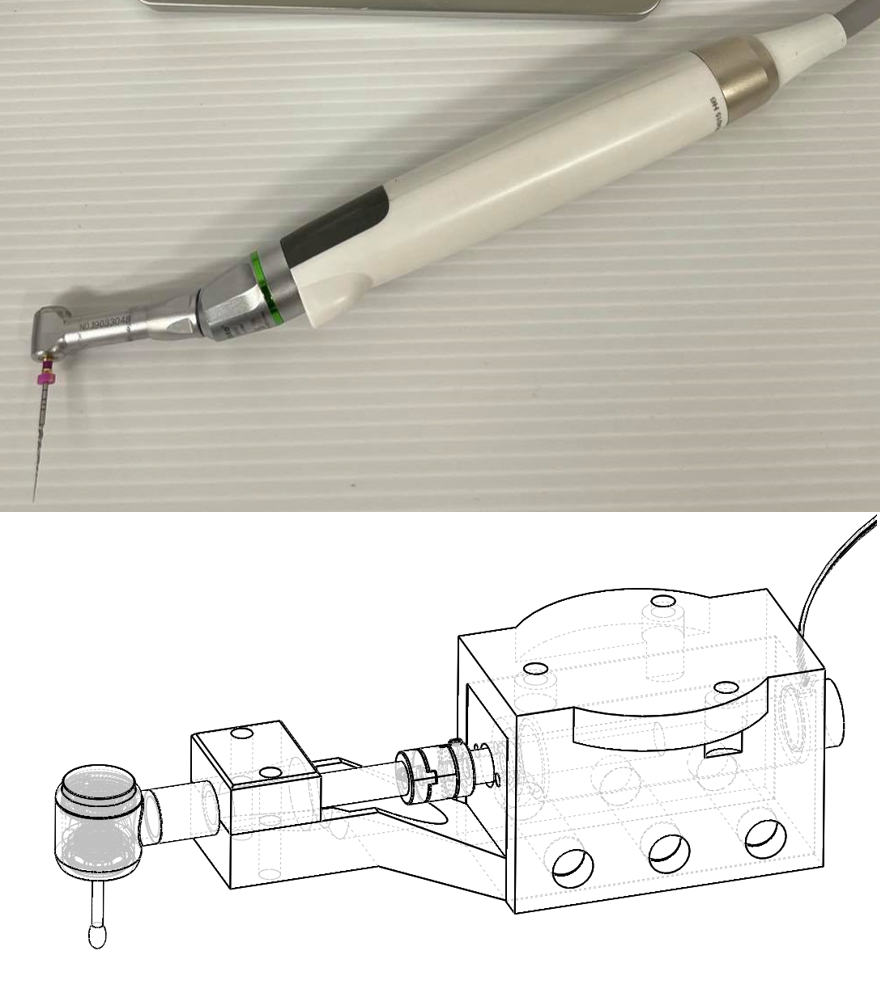
\includegraphics[width=0.7\linewidth]{Images/modified_handpiece.png}
\caption{
Modified dental handpiece composed of a servo motor, a coupler, and the endodontic file.
}\label{fig:modified_handpiece}
\end{center}
\end{figure}	
\par\noindent
A coupler connects the existing handpiece and a servo motor so that the rotation of endodontic file is driven by the servo motor. There is a concern about assembly error because the coupler cannot maintain the motor and the existing hadnpiece in a straight line. The modified handpiece with a motor total weighs around $139$ grams including the adapter used to assemble the F/T sensor and the handpiece. The weight of the modified handpiece is acceptable for the overloads of the F/T sensor and the robot arm.
\par
In conclusion, DentiBot totally has seven degrees of freedom. Six degree of freedom come from Meca500, and the other is from the motor inside our modified handpiece. The rotation of the root canal file is driven by a servo motor, whose maximum rotation speed is around $200$ rpm. The maximum rotation speed - $200$ rpm is lower than the typical standard for endodontic treatment - $300 \sim 600$ rpm. However, the clinical outcome of our proposed algorithm with $200$ rpm is acceptable. It will be proven in Chapter \ref{chapter6}. If needed, the rotation speed can be more faster by changing a higher quality motor.
\newpage													
\section{Kinematics Analysis}
\label{sec:kinematics}
\hspace*{6mm}In this section, coordinate definition is depicted followed by forward kinematics and Jacobian matrix.
\subsection*{Coordinate Definition}
\begin{figure}[htbp]
\begin{center}
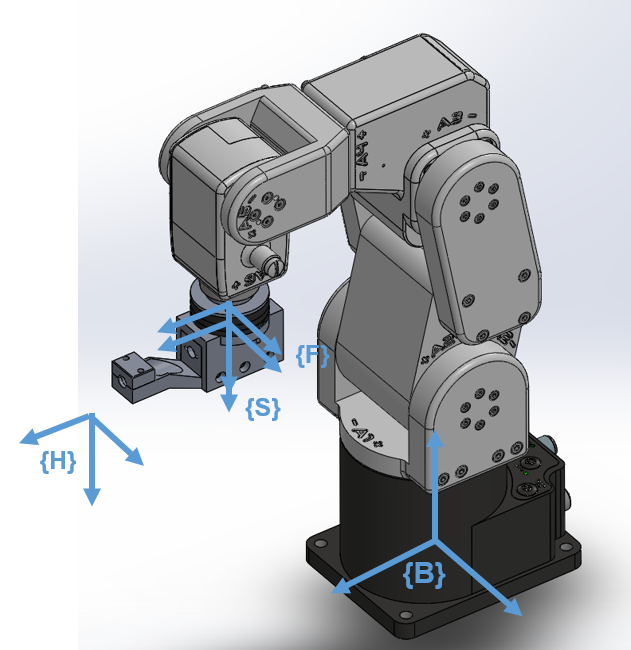
\includegraphics[width=0.85\linewidth]{Images/Coordinates.png}
\caption{
Coordinate definition of DentiBot. \{0\} to \{6\} represent frames of  robot arm axes. \{S\} represents the frame of F/T sensor. \{H\} represents the handpiece tool-tip frame.
}\label{fig:frames}
\end{center}
\end{figure} 

\begin{table}[htbp]
\centering
\caption{Denavit-Hartenberg parameters of Meca500}
\label{tab:DHtable}
\begin{tabular}{ccccc} 
\hline \hline
$i$ (link number)		&$\alpha _{i-1}$ (deg)	&$a_{i-1}$ (mm)	& $\theta _i$ (deg)			&$d_i$ (mm)	\\
\hline
1   					&0    					&0				&$\theta _1$				&135 \\
2   					&-90   					&0				&$\theta _2-90$				&0 \\
3  						&0    					&135			&$\theta _3$ 				&0 \\
4   					&-90    				&38				&$\theta _4$ 				&120 \\
5   					&90   					&0				&$\theta _5$ 				&0 \\
6						&-90  					&0				&$\theta _6+180$ 				&70 \\
\hline\hline
\end{tabular}
\end{table}
\subsection*{Forward Kinematics}
\label{sec:forward}
\hspace*{6mm}Denavit-Hartenberg parameters are shown as Table \ref{tab:DHtable}. Then, the forward kinematics of Meca500 is derived as
\begin{equation}
\label{eq:translation matrix}
\begin{split}
^0_6\mathbf{T} =
\ ^0_1\mathbf{T} \cdot \ ^1_2\mathbf{T} \cdot \ ^2_3\mathbf{T} \cdot \ ^3_4\mathbf{T} \cdot \ ^4_5\mathbf{T} \cdot \ ^5_6\mathbf{T} =
\begin{bmatrix}
^0_6\mathbf{R}	&^0\boldsymbol{p}_\mathrm{6}\\
0				&1\\
\end{bmatrix}\\
\end{split}
\end{equation}
where $^0_6\mathbf{R}$ is the rotation matrix from frame\{6\} to frame\{0\}, $^0\boldsymbol{p}_\mathrm{6}$ is the origin of the frame\{6\} observed from frame\{0\}. All detailed indexes of $^0_6\mathbf{T}$ are shown in Appendix A.
\par
By the way, there is an alternative to calculate the transformation matrix $^0_6\mathbf{T} $ in real-time. The robot arm command -- GetPose -- provide position information ($x$, $y$, $z$, $\alpha$, $\beta$, $\gamma$). ($x$, $y$, $z$) is exactly $^0\boldsymbol{p}_\mathrm{6}$. $(\alpha$, $\beta$, $\gamma)$ are Euler angles and denote (raw, pitch, yaw).  Hence, we can use these information to derive the following equation.
\begin{equation}
\begin{split}
^0_6\mathbf{T} 
&=
\begin{bmatrix}
^0_6\mathbf{R}	&^0\boldsymbol{p}_\mathrm{6}\\
0				&1\\
\end{bmatrix}\\
&= 
\begin{bmatrix}
\mathbf{R}_x(\alpha ) \cdot \mathbf{R}_y(\beta ) \cdot \mathbf{R}_z(\gamma ) 
& \begin{matrix}
x\\ 
y\\ 
z
\end{matrix}\\ 
0 & 1
\end{bmatrix}\\
&= 
\begin{bmatrix} 
C_\beta C_\gamma 										& -C_\beta S_\gamma 									& S_\beta 					&x\\ 
C_\alpha S_\gamma +  S_\alpha S_\beta C_\gamma 			& C_\alpha C_\gamma -  s_\alpha S_\beta S_\gamma		& -S_\alpha C_\beta			&y\\ 
S_\alpha S_\gamma -  C_\alpha S_\beta C_\gamma 			& S_\alpha C_\gamma +  C_\alpha S_\beta S_\gamma 		& C_\alpha C_\beta 			&z\\ 
0 														&0 														&0							&1
\end{bmatrix}
\end{split}
\end{equation}
where $C_{\star} $, $ S_{\star}$ denote $\cos \left(\star \right)$, $\sin \left(\star \right)$; $\alpha ,\beta ,\gamma$ are in representation of Euler angles.
\subsection*	{Jacobian matrix} 
\label{sec:jacobian}
\hspace*{6mm}Jacobian matrix has geometric Jacobian and analytical Jacobian. Therefore, geometric Jacobian based on frame\{0\}, geometric Jacobian based on frame\{H\}, and analytical Jacobian are evaluated in this subsection.
\subsubsection{Geometric Jacobian Based on Frame\{0\}}
\hspace*{6mm}\
First, we should clarify the difference between geometric Jacobian and analytical Jacobian. They both use the same linear velocity but different angular velocity. The angular velocity which geometric Jacobian applies is relevant to the angular velocity ($\theta _x$, $\theta _y$, $\theta _z$). In contrast, the angular velocity which analytical Jacobian contemplates is related to the orientation ($\alpha$, $\beta$, $\gamma$) of the end effector. Therefore, the geometric Jacobian has a clear physical meaning due to the differential ($\theta _x$, $\theta _y$, $\theta _z$) is the angular velocity . Besides, because the geometric Jacobian can be considered in different frames, it is important to clearly understand and familiar with which frame is our option.
\par
Before examining the geometric Jacobian matrix, it will be necessary to find the relationship between the position and joints' angles and the relationship between the angular velocity and the joints' angles.
\par
Based on the translation matrix in Equation \ref{eq:translation matrix}, we obtain the relationship between the position and joints' angles.
\begin{equation}
\label{eq:lin vel}
\begin{split}
^0\boldsymbol{p}_\mathrm{6}
= 
\begin{bmatrix}
x\\
y\\
z\\
\end{bmatrix} 
=
\begin{bmatrix}
x(\theta _1, \theta _2, \cdots, \theta _6)\\
y(\theta _1, \theta _2, \cdots, \theta _6)\\
z(\theta _1, \theta _2, \cdots, \theta _6)
\end{bmatrix} 
\end{split}
\end{equation}
Moreover, the relationship between the angular velocity and derivative of joints' angles is 
\begin{equation}
\label{eq:ang vel_axis}
\begin{split}
\begin{bmatrix}
\theta _x \\
\theta _y \\
\theta _z 
\end{bmatrix}
=
\ ^0_1\mathbf{R}
\begin{bmatrix}
0 \\ 
0 \\ 
\theta _1
\end{bmatrix}
+
\ ^0_2\mathbf{R}
\begin{bmatrix}
0 \\ 
0 \\ 
\theta _2
\end{bmatrix}
+
\ ^0_3\mathbf{R}
\begin{bmatrix}
0 \\ 
0 \\ 
\theta _3
\end{bmatrix}
+
\ ^0_4\mathbf{R}
\begin{bmatrix}
0 \\ 
0 \\ 
\theta _4
\end{bmatrix}
+
\ ^0_5\mathbf{R}
\begin{bmatrix}
0 \\ 
0 \\ 
\theta _5
\end{bmatrix}
+
\ ^0_6\mathbf{R}
\begin{bmatrix}
0 \\ 
0 \\ 
\theta _6
\end{bmatrix}
\end{split}
\end{equation}
Therefore, Jacobian matrices can be obtained by differentiating Equation \ref{eq:lin vel} and \ref{eq:ang vel_axis} as following equation
\begin{equation}
\begin{split}
\boldsymbol{v} 
&= 
\begin{bmatrix}
\dot{x}\\
\dot{y}\\
\dot{z}
\end{bmatrix}
=
\mathbf{J_{gv}} \cdot \boldsymbol{\dot{\theta}}
\\
\boldsymbol{w} 
&= 
\begin{bmatrix}
\dot{\theta _x}\\
\dot{\theta _y}\\
\dot{\theta _z}
\end{bmatrix}
=
\mathbf{J_{gw}} \cdot \boldsymbol{\dot{\theta}}
\end{split}
\end{equation}
where
\begin{equation*}
\begin{split}
\mathbf{J_{gv}} =
\begin{bmatrix}
\frac{\partial x}{\partial \theta _1}	&\frac{\partial x}{\partial \theta _2}	&\cdots		&\frac{\partial x}{\partial \theta _6}\\
\frac{\partial y}{\partial \theta _1}	&\frac{\partial y}{\partial \theta _2}	&\cdots		&\frac{\partial y}{\partial \theta _6}\\
\frac{\partial z}{\partial \theta _1}	&\frac{\partial z}{\partial \theta _2}	&\cdots		&\frac{\partial z}{\partial \theta _6}
\end{bmatrix}
,\ \mathbf{J_{gw}} = 
\begin{bmatrix}
\frac{\partial \theta _x}{\partial \theta _1}	&\frac{\partial \theta _x}{\partial \theta _2}	&\cdots		&\frac{\partial \theta _x}{\partial \theta _6}\\
\frac{\partial \theta _y}{\partial \theta _1}	&\frac{\partial \theta _y}{\partial \theta _2}	&\cdots		&\frac{\partial \theta _y}{\partial \theta _6}\\
\frac{\partial \theta _z}{\partial \theta _1}	&\frac{\partial \theta _z}{\partial \theta _2}	&\cdots		&\frac{\partial \theta _z}{\partial \theta _6}
\end{bmatrix} 
,\ \boldsymbol{\dot{\theta}}
=
\begin{bmatrix}
\dot{\theta _1} \\ 
\dot{\theta _2} \\ 
\dot{\theta _3} \\ 
\dot{\theta _4} \\ 
\dot{\theta _5} \\ 
\dot{\theta _6} 
\end{bmatrix}\\
\end{split}
\end{equation*}
Then, the geometric Jacobian matrix based on frame\{0\} $\mathbf{^0J_g}$ is derived as
\begin{equation}
\begin{split}
\mathbf{^0J_g}
=
\begin{bmatrix}
\mathbf{J_{gv}}\\
\mathbf{J_{gw}}
\end{bmatrix}_{(6 \times 6)}
\end{split}
\end{equation}
Finally, a relationship between $\boldsymbol{\dot{x}}$ and $\boldsymbol{\dot{\theta}}$ is derived as 
\begin{equation}
\label{eq:jg0}
\begin{split}
\boldsymbol{\dot{x}} &= \ \mathbf{^0\!J_g} \cdot \boldsymbol{\dot{\theta}} 		\\ 
\boldsymbol{\dot{\theta}} &= \ \mathbf{^0\!J_g^{-1}} \cdot \boldsymbol{\dot{x}}
\end{split}
\end{equation}
where
\begin{equation*}
\begin{split}
\boldsymbol{\dot{x}}
=
\begin{bmatrix}
\dot{x}\\
\dot{y}\\
\dot{z}\\
\dot{\theta _x}\\
\dot{\theta _y}\\
\dot{\theta _z}
\end{bmatrix}_{\!\{0\}}
,\ 
\boldsymbol{\dot{\theta}}
=
\begin{bmatrix}
\dot{\theta _1} \\ 
\dot{\theta _2} \\ 
\dot{\theta _3} \\ 
\dot{\theta _4} \\ 
\dot{\theta _5} \\ 
\dot{\theta _6} 
\end{bmatrix}
\end{split}
\end{equation*}
\par
By extension, in terms of the Jacobian matrix, the property between joint torque and force can be derived as
\begin{equation}
\begin{split}
\boldsymbol{\tau } &= \mathbf{^0\!J^\top _g} \cdot \boldsymbol{f}	\\
\Rightarrow
\begin{bmatrix}
\tau_{\theta _1} \\ 
\tau_{\theta _2} \\ 
\tau_{\theta _3} \\ 
\tau_{\theta _4} \\ 
\tau_{\theta _5} \\ 
\tau_{\theta _6} \\ 
\end{bmatrix}
&=
\mathbf{^0\!J^\top _g} 
\cdot
\begin{bmatrix}
f_x \\ 
f_y \\ 
f_z \\ 
\tau_{x} \\ 
\tau_{y} \\ 
\tau_{z}
\end{bmatrix}
\end{split}
\end{equation}
where $\boldsymbol{\tau }$ is the vector of joints' torques and $\boldsymbol{f}$ is the vector composed of inertial forces and torques of the robot arm.
\subsubsection{Geometric Jacobian Based on Frame\{H\}}
\label{sec:jg6}
\hspace*{6mm}Why the geometric Jacobian based on frame\{H\} $^{\mathrm{H}}\!\mathbf{J_g}$ is important is that in section \ref{sec:adm ctrl} admittance control is applied and use F/T sensor detect forces and torques relative to frame\{H\} instead of frame\{0\}. 
\par
To obtain $^{\mathrm{H}}\!\mathbf{J_g}$, we derive it from $\mathbf{^0\!J_g}$. Therefore, to start with Equation \ref{eq:jg0}.
\begin{equation}
\begin{split}
\begin{bmatrix}
\dot{x}\\
\dot{y}\\
\dot{z}\\
\dot{\theta _x}\\
\dot{\theta _y}\\
\dot{\theta _z}
\end{bmatrix}_{\!\{0\}}
=
\mathbf{^0\!J_g} \cdot 
\begin{bmatrix}
\dot{\theta _1} \\ 
\dot{\theta _2} \\ 
\dot{\theta _3} \\ 
\dot{\theta _4} \\ 
\dot{\theta _5} \\ 
\dot{\theta _6} 
\end{bmatrix}\\
\end{split}
\end{equation}
Then, left-multiply an augmented rotation matrix composed of $^{\mathrm{H}}_0\mathbf{R}$.
\begin{equation}
\label{eq:jg6_leftmul}
\begin{split}
\begin{bmatrix}
^{\mathrm{H}}_0\mathbf{R} & 0_{ 3\times 3} \\ 
0_{ 3\times 3} & ^{\mathrm{H}}_{0}\mathbf{R}
\end{bmatrix}
\cdot
\begin{bmatrix}
\dot{x}\\
\dot{y}\\
\dot{z}\\
\dot{\theta _x}\\
\dot{\theta _y}\\
\dot{\theta _z}
\end{bmatrix}_{\!\{0\}}
=
\begin{bmatrix}
^{\mathrm{H}}_0\mathbf{R} & 0_{ 3\times 3} \\ 
0_{ 3\times 3} & ^{\mathrm{H}}_{0}\mathbf{R}
\end{bmatrix}
\cdot
\mathbf{^0\!J_g} \cdot 
\begin{bmatrix}
\dot{\theta _1} \\ 
\dot{\theta _2} \\ 
\dot{\theta _3} \\ 
\dot{\theta _4} \\ 
\dot{\theta _5} \\ 
\dot{\theta _6} 
\end{bmatrix}\\
\end{split}
\end{equation}
Since the transformation coordinate relationship between frame\{0\} and frame\{6\} is 
\begin{equation}
\label{eq: t06}
\begin{split}
\begin{bmatrix}
\dot{x}\\ 
\dot{y}\\ 
\dot{z}\\ 
\dot{\theta_x}\\ 
\dot{\theta_y}\\
\dot{\theta_z} 
\end{bmatrix}_{\!\{\mathrm{H}\}}
=
\begin{bmatrix}
^\mathrm{H}_0\mathbf{R} & 0_{ 3\times 3} \\ 
0_{ 3\times 3} & ^\mathrm{H}_0\mathbf{R}
\end{bmatrix}
\begin{bmatrix}
\dot{x}\\ 
\dot{y}\\ 
\dot{z}\\ 
\dot{\theta_x}\\ 
\dot{\theta_y}\\
\dot{\theta_z} 
\end{bmatrix}_{\!\{0\}}
\end{split}
\end{equation}
Substitute Equation \ref{eq: t06} into Equation \ref{eq:jg6_leftmul}.
\begin{equation}
\begin{split}
\begin{bmatrix}
\dot{x}\\
\dot{y}\\
\dot{z}\\
\dot{\theta _x}\\
\dot{\theta _y}\\
\dot{\theta _z}
\end{bmatrix}_{\!\{\mathrm{H}\}}
=
\begin{bmatrix}
^{\mathrm{H}}_0\mathbf{R} & 0_{ 3\times 3} \\ 
0_{ 3\times 3} & ^{\mathrm{H}}_{0}\mathbf{R}
\end{bmatrix}
\cdot
\mathbf{^0\!J_g} \cdot 
\begin{bmatrix}
\dot{\theta _1} \\ 
\dot{\theta _2} \\ 
\dot{\theta _3} \\ 
\dot{\theta _4} \\ 
\dot{\theta _5} \\ 
\dot{\theta _6} 
\end{bmatrix}\\
\end{split}
\end{equation}
Because 
\begin{equation}
\label{eq:jg6}
\begin{split}
\boldsymbol{\dot{x}} &= \ ^{\mathrm{H}}\!\mathbf{J_g} \cdot \boldsymbol{\dot{\theta}}		
\end{split}
\end{equation}
where
\begin{equation*}
\begin{split}
\boldsymbol{\dot{x}}
=
\begin{bmatrix}
\dot{x}\\
\dot{y}\\
\dot{z}\\
\dot{\theta _x}\\
\dot{\theta _y}\\
\dot{\theta _z}
\end{bmatrix}_{\!\{\mathrm{H}\}}
,\ 
\boldsymbol{\dot{\theta}}
=
\begin{bmatrix}
\dot{\theta _1} \\ 
\dot{\theta _2} \\ 
\dot{\theta _3} \\ 
\dot{\theta _4} \\ 
\dot{\theta _5} \\ 
\dot{\theta _6} 
\end{bmatrix}
\end{split}
\end{equation*}
Therefore the relationship between $\mathbf{^\mathrm{H}\!J_g}$ and $\mathbf{^0\!J_g}$ is obtained.
\begin{equation}
\begin{split}
\mathbf{^\mathrm{H}\!J_g}
= 
\begin{bmatrix}
^{\mathrm{H}}_0\mathbf{R} & 0_{ 3\times 3} \\ 
0_{ 3\times 3} & ^{\mathrm{H}}_0\mathbf{R}
\end{bmatrix}
\cdot
\mathbf{^0\!J_g}
\end{split}
\end{equation}
In conclusion, $^{\mathrm{H}}\!\mathbf{J_g}$ can be derived from $\mathbf{^0\!J_g}$, and then we can analyze kinematics on frame\{H\} with $^{\mathrm{H}}\!\mathbf{J_g}$.
\subsubsection{Analytical Jacobian}
\hspace*{6mm}The linear velocity of analytical Jacobian and geometric Jacobian is the same as shown in Equation \ref{eq:lin vel}. Nevertheless, as for angular velocity, analytical Jacobian takes the orientation ($\alpha$, $\beta$, $\gamma$) of the end effector into consideration. 
\par
Analytical Jacobian can be derived from geometric Jacobian. First, we investigate the relationship between the angular velocity and derivative of orientation of the end effector as following.
\begin{equation}
\label{eq: Jwe}
\begin{split}
\begin{bmatrix}
\theta _x \\ 
\theta _y \\ 
\theta _z
\end{bmatrix}
&=
\begin{bmatrix}
\alpha \\ 
0\\ 
0
\end{bmatrix}
+
\mathbf{R}_x(\alpha )
\begin{bmatrix}
0 \\ 
\beta \\ 
0
\end{bmatrix}
+
\mathbf{R}_x(\alpha )\mathbf{R}_y(\beta )
\begin{bmatrix}
0 \\ 
0\\ 
\gamma
\end{bmatrix}\\
&=
\begin{bmatrix}
1 & 0 & S_\beta \\ 
0 & C_\alpha & -S_\alpha C_\beta \\ 
0 & S_\alpha & C_\alpha C_\beta
\end{bmatrix}
\begin{bmatrix}
\alpha \\ 
\beta\\ 
\gamma
\end{bmatrix}
\end{split}
\end{equation}
Then, utilize this generalized vector to get its Jacobian matrix $\mathbf{J_{we}}$.
\begin{equation}
\begin{split}
\begin{bmatrix}
\dot{\theta _x} \\ 
\dot{\theta _y} \\ 
\dot{\theta _z}
\end{bmatrix}
=
\mathbf{J_{\!we}}
\cdot
\begin{bmatrix}
\dot{\alpha} \\ 
\dot{\beta} \\ 
\dot{\gamma}
\end{bmatrix}
\end{split}
\end{equation}
where
\begin{equation*}
\label{eq:jacobian_euler}
\begin{split}
\mathbf{J_{we}}
=
\begin{bmatrix}
1														& \gamma C_{\beta}							& S_{\beta}\\
- \beta S_{\alpha} -  \gamma C_{\alpha}C_{\beta}		& C_{\alpha} +  \gamma S_{\alpha}S_{\beta}	& -C_{\beta}S_{\alpha}\\
\beta C_{\alpha} -  \gamma C_{\beta}S_{\alpha}			& S_{\alpha} -  \gamma C_{\alpha}S_{\beta}	&  C_{\alpha}C_{\beta}
\end{bmatrix}
\end{split}
\end{equation*}
Therefore,
\begin{equation}
\begin{split}
\begin{bmatrix}
\dot{x} \\
\dot{y} \\
\dot{z} \\
\dot{\theta _x} \\
\dot{\theta _y} \\
\dot{\theta _z} 
\end{bmatrix}
=
\begin{bmatrix}
\mathbf{I}_{3\times 3} & 0_{3\times 3}\\
0_{3\times 3} & \mathbf{J_{we}}
\end{bmatrix}
\begin{bmatrix}
\dot{x} \\
\dot{y} \\
\dot{z} \\
\dot{\alpha} \\ 
\dot{\beta} \\ 
\dot{\gamma} 
\end{bmatrix}
\end{split}
\end{equation}
Finally, we obtain the relationship between geometric and analytical Jacobian.
\begin{equation}
\begin{split}
\mathbf{J_g} &= 
\begin{bmatrix}
\mathbf{I}_{3\times 3} & 0_{3\times 3}\\
0_{3\times 3} & \mathbf{J_{we}}
\end{bmatrix}
\mathbf{J_a}
\\
\mathbf{J_a} &= 
\begin{bmatrix}
\mathbf{I}_{3\times 3} & 0_{3\times 3}\\
0_{3\times 3} & \mathbf{J_{we}^{-1}}
\end{bmatrix}
\mathbf{J_g}
\end{split}
\end{equation}

\section{Tool-tip Coordinate}
\label{sec:ref_robot}
\hspace*{6mm}To obtain translation and rotation vector, we respectively introduce Tool Center Point to find the translation vector and propose an approach to find the rotation vector.				
\subsubsection{Translation Analysis - Tool Center Point}
\label{sec:tcp}
\hspace*{6mm}So far, with the forward and inverse kinematics, the robot arm can translate and rotate around frame\{6\}. However, the origin of the frame\{6\} is not an operating point. Because the F/T sensor and a detachable end effector will be both mounted on the wrist, the tool-tip position is what we want. That means we should let the robot arm know how to translate and rotate in frame\{H\} instead of frame\{6\}. If we have translation and rotation information of the tool-tip, there is an easy way to directly give the above information to the robot arm. SetTRF ($x$, $y$, $z$, $\alpha$, $\beta$, $\gamma$) is the command of the robot arm, whose ($x$, $y$, $z$) is translation vector and ($\alpha$, $\beta$, $\gamma$) is rotation vector in representation of Euler angles.
\par
Tool Center Point (TCP) is a critical problem for robot arm control \cite{yang2017four}. In the previous section, the forward kinematics of the robot arm have evaluated. By Calculating kinematics, The robot arm can keep track of the origin of the frame\{6\}, which is observed from the base frame. The robot arm has the capability to translate and rotate with the origin of the frame\{6\}. The above motions are like a remote center motion (RCM).  Nevertheless, it's inefficient to recalculate the transformation matrix via mechanism dimension when changing an end effector or a tool (endodontic file). Besides, using forward kinematics to find the tool-tip frame can not avoid assembly errors.
\begin{figure}[htbp]
\begin{center}
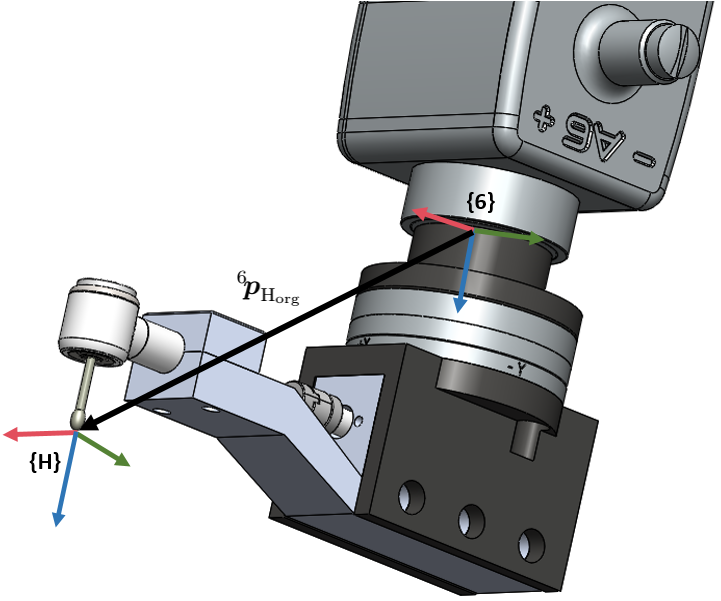
\includegraphics[width=0.7\linewidth]{Images/TCP.png}
\caption{
Schematic diagram for tool center point (TCP). The translation vector $^\mathrm{6}\!\boldsymbol{p}_\mathrm{H}$ denotes the origin position relative to the frame\{6\}.
}\label{fig:tcp}
\end{center}
\end{figure}
\par
In order to overcome this problem, the four-points method is interpreted to obtain the tool-tip position information, which is also the translation vector. From Figure \ref{fig:frames}, the transformation matrix between the frame\{0\} and frame\{H\} is evaluated as 
\begin{equation}
\begin{split}
_{\mathrm{H}}^{\mathrm{0}}\mathbf{T} &=\ _{\mathrm{6}}^{\mathrm{0}}\mathbf{T}\cdot \ _{\mathrm{H}}^{\mathrm{6}}\mathbf{T}\\
\end{split}
\end{equation}		
and can be rewritten as
\begin{equation}
\begin{split}																												
\begin{bmatrix}
_{\mathrm{H}}^{\mathrm{0}}\mathbf{R} & ^\mathrm{0}\!\boldsymbol{p}_\mathrm{H}\\ 
0 & 1
\end{bmatrix} &=
\begin{bmatrix}
_{\mathrm{6}}^{\mathrm{0}}\mathbf{R} & ^\mathrm{0}\!\boldsymbol{p}_\mathrm{6}\\ 
0 & 1
\end{bmatrix}
\begin{bmatrix}
_{\mathrm{H}}^{\mathrm{6}}\mathbf{R} & ^\mathrm{6}\!\boldsymbol{p}_\mathrm{H}\\ 
0 & 1
\end{bmatrix}\\
%----------------------------------------------------------------------------------------------------------------------------
&= 
\begin{bmatrix}
_{\mathrm{6}}^{\mathrm{0}}\mathbf{R} \cdot _{\mathrm{H}}^{\mathrm{6}}\!\mathbf{R} & _{\mathrm{6}}^{\mathrm{0}}\mathbf{R} \cdot ^\mathrm{6}\!\!\boldsymbol{p}_\mathrm{H} +\ ^\mathrm{0}\!\boldsymbol{p}_\mathrm{6}\\ 
0 & 1
\end{bmatrix}\\
\end{split}
\end{equation}
where $\mathbf{R}$ is the rotation matrix, $^0\boldsymbol{p}_\mathrm{6}$ is the origin of the frame\{6\} observed from frame\{0\}, and $^\mathrm{6}\!\boldsymbol{p}_\mathrm{H}$ is the origin of the frame\{H\} observed from frame\{6\}.
Consequently, a crucial equation is obtained
\begin{equation}
\begin{split}
^\mathrm{0}\!\boldsymbol{p}_\mathrm{H} &=\  _{\mathrm{6}}^{\mathrm{0}}\mathbf{R}\cdot\ ^\mathrm{6}\!\boldsymbol{p}_\mathrm{H} +\ ^\mathrm{0}\!\boldsymbol{p}_\mathrm{6}\\
\end{split}
\end{equation}
\par\noindent
Now, we move the tool-tip to a fixed point with four different poses including position and orientation as shown in Figure \ref{fig:four point}. Then, four different rotation matrices and vectors are derived. 
\begin{equation}
\label{eq:four-points}
\begin{split}			
^\mathrm{0}\!\boldsymbol{p}_\mathrm{H}&=\  _{\mathrm{6}}^{\mathrm{0}}\mathbf{R}^1 \cdot\ ^\mathrm{6}\!\boldsymbol{p}_\mathrm{H} +\ ^\mathrm{0}\!\boldsymbol{p}_\mathrm{6}^1\\
%----------------------------------------------------------------------------------------------------------------------------
					  						&=\  _{\mathrm{6}}^{\mathrm{0}}\mathbf{R}^2 \cdot\ ^\mathrm{6}\!\boldsymbol{p}_\mathrm{H} +\ ^\mathrm{0}\!\boldsymbol{p}_\mathrm{6}^2\\
%----------------------------------------------------------------------------------------------------------------------------
					  						&=\  _{\mathrm{6}}^{\mathrm{0}}\mathbf{R}^3 \cdot\ ^\mathrm{6}\!\boldsymbol{p}_\mathrm{H} +\ ^\mathrm{0}\!\boldsymbol{p}_\mathrm{6}^3\\
%----------------------------------------------------------------------------------------------------------------------------
					 					 	&=\  _{\mathrm{6}}^{\mathrm{0}}\mathbf{R}^4 \cdot\ ^\mathrm{6}\!\boldsymbol{p}_\mathrm{H} +\ ^\mathrm{0}\!\boldsymbol{p}_\mathrm{6}^4\\
%----------------------------------------------------------------------------------------------------------------------------
\end{split}
\end{equation}
\begin{figure}[htbp]
\begin{center}
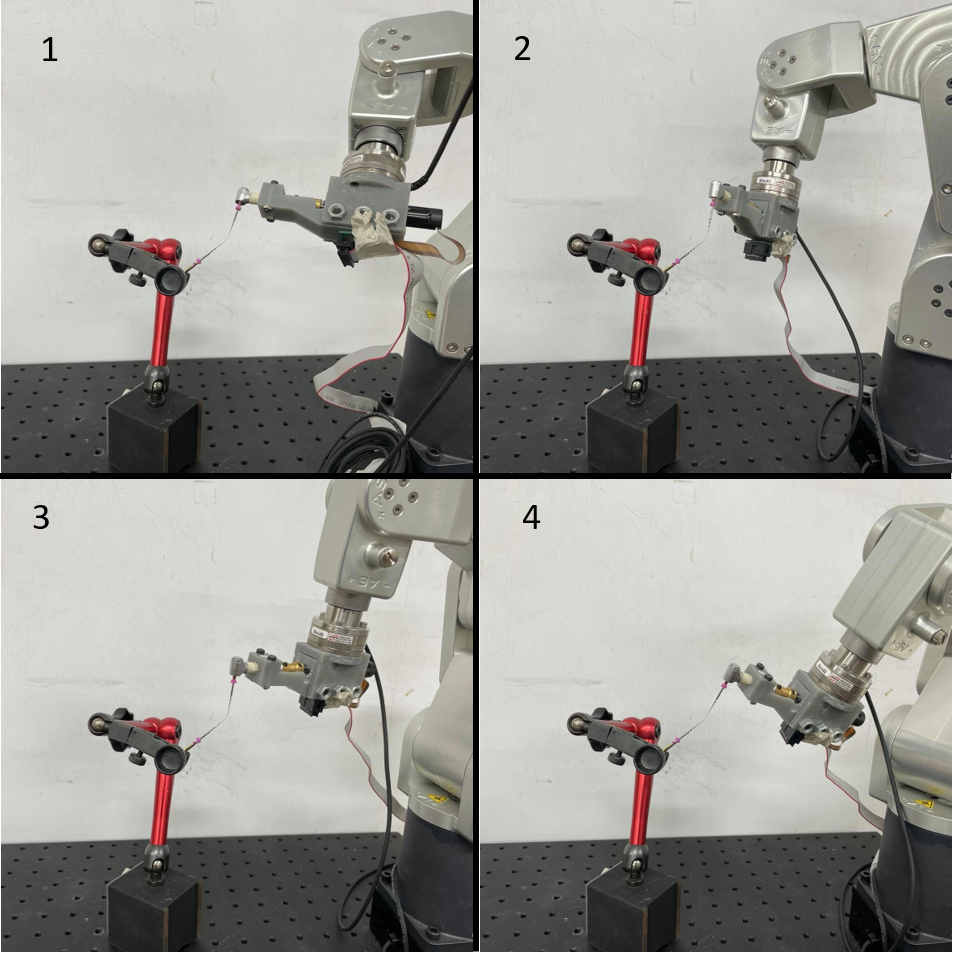
\includegraphics[width=0.55\linewidth]{Images/four point.png}
\caption{
Four points method. Align a fixed point with four different poses.
}\label{fig:four point}
\end{center}
\end{figure}
\newpage
\noindent
$^\mathrm{6}\!\boldsymbol{p}_\mathrm{H}$ is unknown. In order to extract $^\mathrm{6}\!\boldsymbol{p}_\mathrm{H}$ from Equation \ref{eq:four-points}, we subtract the second to forth equation from the first equation.
\begin{equation}
\begin{split}	
\begin{bmatrix}
\  _{\mathrm{6}}^{\mathrm{0}}\mathbf{R}^{1} - \  _{\mathrm{6}}^{\mathrm{0}}\mathbf{R}^{2}\\ 
\  _{\mathrm{6}}^{\mathrm{0}}\mathbf{R}^{1} - \  _{\mathrm{6}}^{\mathrm{0}}\mathbf{R}^{3}\\ 
\  _{\mathrm{6}}^{\mathrm{0}}\mathbf{R}^{1} - \  _{\mathrm{6}}^{\mathrm{0}}\mathbf{R}^{4}
\end{bmatrix}
\cdot\ ^\mathrm{6}\!\boldsymbol{p}_\mathrm{H}
=
\begin{bmatrix}
\ ^\mathrm{0}\!\boldsymbol{p}_\mathrm{6}^{2} -\ ^\mathrm{0}\!\boldsymbol{p}_\mathrm{6}^{1} \\ 
\ ^\mathrm{0}\!\boldsymbol{p}_\mathrm{6}^{3} -\ ^\mathrm{0}\!\boldsymbol{p}_\mathrm{6}^{1} \\ 
\ ^\mathrm{0}\!\boldsymbol{p}_\mathrm{6}^{4} -\ ^\mathrm{0}\!\boldsymbol{p}_\mathrm{6}^{1} 
\end{bmatrix}
\end{split}
\end{equation}
where we define
\begin{equation*}
\begin{split}
\mathbf{R} =  
\begin{bmatrix}
\  _{\mathrm{6}}^{\mathrm{0}}\mathbf{R}^{1} - \  _{\mathrm{6}}^{\mathrm{0}}\mathbf{R}^{2}\\ 
\  _{\mathrm{6}}^{\mathrm{0}}\mathbf{R}^{1} - \  _{\mathrm{6}}^{\mathrm{0}}\mathbf{R}^{3}\\ 
\  _{\mathrm{6}}^{\mathrm{0}}\mathbf{R}^{1} - \  _{\mathrm{6}}^{\mathrm{0}}\mathbf{R}^{4}
\end{bmatrix}_{9 \times 3}, 
\boldsymbol{p} = 
\begin{bmatrix}
\ ^\mathrm{0}\!\boldsymbol{p}_\mathrm{6}^{2} -\ ^\mathrm{0}\!\boldsymbol{p}_\mathrm{6}^{1} \\ 
\ ^\mathrm{0}\!\boldsymbol{p}_\mathrm{6}^{3} -\ ^\mathrm{0}\!\boldsymbol{p}_\mathrm{6}^{1} \\ 
\ ^\mathrm{0}\!\boldsymbol{p}_\mathrm{6}^{4} -\ ^\mathrm{0}\!\boldsymbol{p}_\mathrm{6}^{1} 
\end{bmatrix}_{9 \times 1}
\end{split}
\end{equation*}
Therefore,
\begin{equation*}
\begin{split}
^\mathrm{6}\!\boldsymbol{p}_\mathrm{H} 	&= \mathbf{R}^{\dagger} \cdot \boldsymbol{p}\\
					  							&= \left( \mathbf{R}^\top\mathbf{R}\right) ^{-1}\mathbf{R}^\top \cdot \boldsymbol{p}
\end{split}
\end{equation*}
Finally, we can utilize the four-points method to obtain the translation vector $^\mathrm{6}\!\boldsymbol{p}_\mathrm{H} $.
\subsubsection{Rotation Analysis}
\label{sec:rot inf}
\hspace*{6mm}Turning now to the discussion about the rotation vector. Above all, the vector of tool insertion direction $\boldsymbol{t}$ should be obtained. By applying the TCP method with two endodontic files with different lengths, two vectors $^\mathrm{6}\!\boldsymbol{p}_\mathrm{H_{long}} ,\ ^\mathrm{6}\!\boldsymbol{p}_\mathrm{H_{short}}$ are obtained and illustrated as Figure \ref{fig:tcp2}. Hence, 
\begin{equation}
\begin{split}
\boldsymbol{t} =\ ^\mathrm{6}\!\boldsymbol{p}_\mathrm{H_{long}} -\ ^\mathrm{6}\!\boldsymbol{p}_\mathrm{H_{short}}
\end{split}
\end{equation}
\begin{figure}[htbp]
\begin{center}
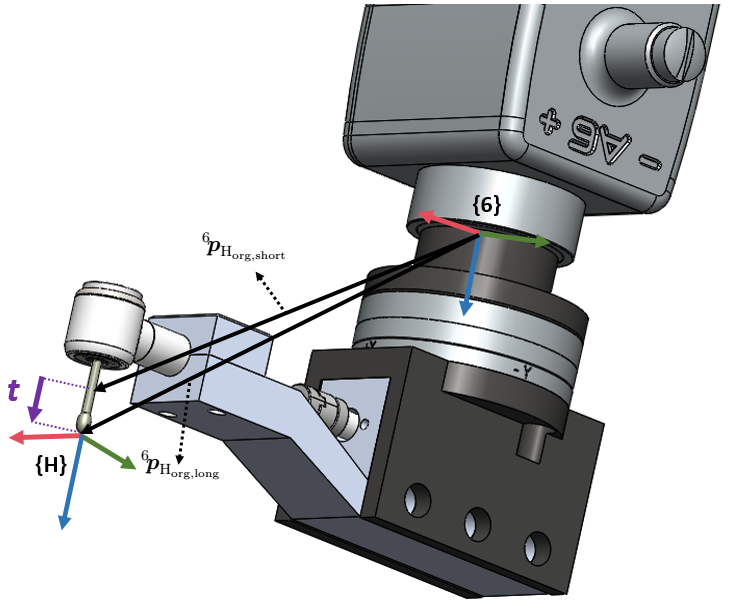
\includegraphics[width=0.7\linewidth]{Images/TCP2.png}
\caption{ 
Schematic diagram for obtaining the tool vector. 
}\label{fig:tcp2}
\end{center}
\end{figure}
\begin{figure}[htbp]
\begin{center}
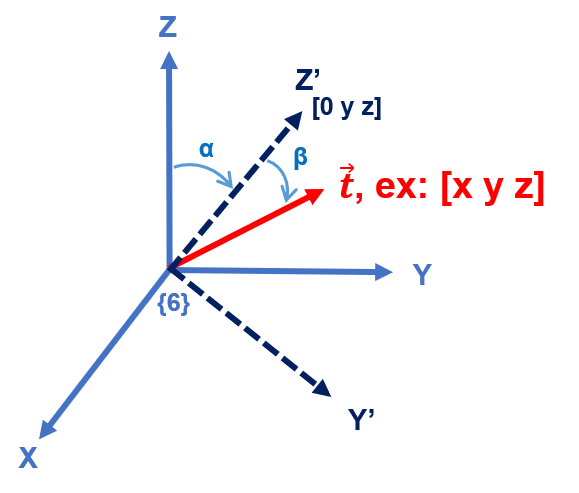
\includegraphics[width=0.6\linewidth]{Images/rot_inf.png}
\caption{
Illustration of finding the rotation matrix with the tool vector
}\label{fig:rot_inf}
\end{center}
\end{figure} 
\par
For analyzing it easily, we depict it in Figure \ref{fig:rot_inf}. Note that here we only discuss rotation, so we assume that we have done translation and matched the frame\{H\} with frame\{6\}. Because we hope to send a Z-axis command to achieve tool insertion, we should align the original Z-axis to the tool vector $\boldsymbol{t}$. Nevertheless, Z-axis alignment without other restrictions will produce many solutions. We choose one of the solutions to align Z-axis to the tool vector. According to the figure, we assume the tool vector $\boldsymbol{t}$ is [$t_x$ $t_y$ $t_z$], whose projection to yz-plane $\mathrm{proj_{(y-z)}}\boldsymbol{t}$ is [0 $t_y$ $t_z$]. Initially, we rotate $\alpha$ degree around X-axis to make original Z-axis align the projection [$0$ $y$ $z$]. Next, we rotate $\beta$ degree around Y' axis and finally align the original Z-axis to the tool vector [$t_x$ $t_y$ $t_z$]. Therefore, 
\begin{equation}
\begin{split}
\ \  _{\mathrm{6}}^{\mathrm{H}}\mathbf{R} = \mathbf{R}_x(\alpha )\mathbf{R}_y(\beta )
\end{split}
\end{equation}
, and 
\begin{equation}
\begin{split}
\alpha &= 
-\mathrm{sign}(t_y)\cdot \cos^{-1} \left(  \frac{\hat{k}						\cdot 		\mathrm{proj_{(y-z)}}\boldsymbol{t}				}
								 				{\left \| \hat{k} \right \| 	\cdot \left \| \mathrm{proj_{(y-z)}}\boldsymbol{t} \right \|} \right)\ \\
\beta  &= 
\mathrm{sign}(t_x)\cdot \cos^{-1} \left( \frac{\textbf{t}							\cdot 		\mathrm{proj_{(y-z)}}\boldsymbol{t}			}
								  			  {\left \| \textbf{t}\right \| 	\cdot \left \| \mathrm{proj_{(y-z)}}\boldsymbol{t} \right \|} \right)\ 
\end{split}
\end{equation}
where $\alpha,\beta$ are Euler angles which could be applied with the robot command "SetTCP", $\hat{k}$ is the unit vector of in the direction of the z-axis, and $\boldsymbol{t}$, [$t_x$ $t_y$ $t_z$], is the tool vector.
%\par
%Assume $\boldsymbol{t} = $ [$x$ $y$ $z$] ,
%\begin{equation}
%\begin{split}
%\alpha &= 
%-\mathrm{sign}(y)\cdot \cos^{-1}	\left( \frac{z^2}{\sqrt{y^2+z^2}} \right) \mathrm\\
%\beta  &= 
%\mathrm{sign}(x)\cdot \cos^{-1} \left( \frac{y^2+z^2}{\sqrt{x^2+y^2+z^2}\sqrt{x^2+y^2+z^2}} \right) \mathrm
%\end{split}
%\end{equation}
%$\alpha$ and $\beta$ are Euler angles, which meet the command demand.
\par
In this section, we have demonstrated two key aspects of reference frame changing of the robot arm. By the translation and rotation information, it's easy to input the results of them via the command setTRF. The robot arm can recognize frame\{H\}, then translate and orientate along with frame\{H\}. Having discussed how to combine a robot arm with an end effector, the next section addresses ways of combining an F/T sensor.